\chapter{Introduction}


Prediction of molecular properties allows the filtering of molecular data sets, 
resulting in fewer wet lab experiments and a reduced development time of novel 
drugs and materials.\cite{adelusi2022molecular} However, ab initio quantum chemical algorithms are currently 
intractable due to their high computational cost.\cite{szabo2012modern} Therefore, more efficient 
algorithms are necessary, considering that the chemical space of drugable molecules 
is estimated to be $10^{60}$. One approach is machine learning (ML) algorithms, as these 
algorithms can find complicated patterns in large data sets.\cite{gorgulla2022emerging} The problem with ML 
algorithms is their black-box nature, which limits the creation of novel scientific 
knowledge and can result in trust issues in performance-critical and highly regulated 
environments.\cite{carvalho2019machine}


Explainable artificial intelligence (XAI) tries to get insight into black-box 
ML models.\cite{carvalho2019machine, yuan2022explainability} 
Current XAI methods focus on the ML model and often neglect domain 
knowledge of the studied problem. For example, when molecules are represented 
as graphs using the Lewis structure\cite{ahmad1992drawing}, common XAI techniques will search for the 
most important nodes or subgraphs to explain molecular property prediction.\cite{wu2023chemistry} The 
resulting explanation, however, is not chemically relevant as chemists are used 
to thinking in terms of substructures such as functional groups. Recently, Wu et. 
al. developed an attribution based XAI method that first partitions the molecular graph into 
chemically meaningful substructures. Therefore, their method, substructure graph 
exploration (SME), can produce chemically intuitive explanations.\cite{wu2023chemistry}


SME takes the difference between the model prediction of the molecular graph and 
the prediction of the molecular graph in which a substructure is masked. Yet, 
this approach does not consider the interaction between molecular substructures.
A commonly used attribution method in machine learning that does consider 
interactions between features is the Shapley value. Here, the Shapley value\cite{shapley1953value} will 
be used to compute the attributions of molecular graphs using a similar approach 
of Wu et. al. Since the Shapley value does not take the graphical structure of 
the input into account, the Hamiache-Navarro value\cite{hamiache_value_1999} 
is also considered to investigate whether the inclusion of the graphical structure 
can significantly improve the explanation. Comparison of the different attribution 
methods is done using pairwise Spearman rank correlation between attributions of 
different methods. The fidelity\cite{carvalho2019machine} is used to measure 
how faithful the explanation is to the model. Spearman rank correlation is also 
used to compare the ranked attributions to a manual ranks obtained using chemical 
intuition. 


The explanation methods are applied to a machine learning model that predicts the 
estimated water solubility in logS (with S the solubility in $mol/L$). Water 
solubility is chosen as the relative water solubility of a compound can be estimated 
from its molecular structure. Also, the prediction of water solubility is used 
in drugs discovery as this influences the drug blood concentration.\cite{hill2010getting}


\section{Machine learning}


Machine learning algorithms require a feature matrix $\mathbf{X} \in \mathbb{R}^{N \times p}$
where each row represents a sample and each column relates to an attribute. 
Supervised ML additionally requires a target vector $\pmb{y} \in \mathbb{R}^N$
representing another feature with a value for each sample. Then, the goal of an ML method is 
to construct a function $f$, based on parameters $\pmb{\theta}$, that can accurately 
predict the outcome variable $\pmb{y}$ of the training data $\pmb{X}$ and can 
generalize to new data.\cite{hastie2009elements} After obtaining the predicted 
values $\hat{\pmb{Y}} = f\left(\pmb{X}; \pmb{\theta}\right)$, they are compared 
to the true values $\pmb{y}$ (also called labels)
in order to determine how good the model is, which introduces the concept of loss functions $\mathcal{L}$.
Different loss functions exists for different kind of problems.\cite{wang2020comprehensive}
A commonly used loss function is the mean squared error (MSE) (\cref{eq:mse})
which averages the squared difference between the predicted value and true label.
Furthermore, optimizing the loss function with respect to the learning function
parameters produces the best model with the given architecture.\cite{hastie2009elements}


\begin{equation}
	\label{eq:mse}
	\text{MSE}\big(\pmb{y}, \pmb{X}\big) = \frac{1}{N}  \big[\pmb{y} - f(\mathbf{X})\big]^T[\pmb{y} - f(\mathbf{X})\big]
\end{equation}


One of the simplest functions $f\left(\mathbf{X}; \pmb{\theta}\right) = \mathbf{X}\pmb{\theta}$
is a linear combination of the features, where $\pmb{\theta} \in \mathbb{R}^p$
is the vector of coefficients. This model, known as linear regression, is commonly
used in statistical modeling.\cite{kutner2005applied} Although the linear model is
very interpretable, the linearity constraint is too strict which limits its
applicability. Therefore, more complicated ML algorithms were developed which are
able to obtain improved performance on complicated data with respect to linear
regression by allowing non-linear relationships.\cite{deng2012mnist} However,
they pay a price in terms of interpretability.\cite{fan2021interpretability}


\section{Neural networks}


Neural networks (NN) are a class of machine learning algorithms which are able to
approximate complicated non-linear function, inspired by the human brain.
\cite{cybenko1989approximation, rosenblatt1962principles} Although a NN is a strong
simplification of the human brain, the concept of neuron signal transit is used 
as a basic building block.\cite{wang2017origin} This signal transmission
takes place between units in a neural network. Then, different architectures
can be used to connect different units. Rosenblatt proposed a weighted sum 
of the inputs followed by a non-linear activation function.\cite{rosenblatt1962principles}
This neural network is, however, still a linear function due to its inability 
to learn non-linear functions. A solution to this limitation is stacking multiple 
perceptrons after each other, resulting in a multi layer perceptron (MLP).
The multi layer perceptron (MLP) is a basic architecture that is frequently 
utilized in other, more complicated neural networks.\cite{almeida2020multilayer}
In an MLP (\cref{fig:mlp_structure}) three parts can be distinguished: an input layer,
one or more hidden layers and an output layer.


\begin{figure}[h]
	\centering
	\includegraphics[scale=1.5]{mlp.png}
	\caption{General structure of a multi layer perceptron (MLP) consisting of an input layer,
		one or multiple hidden layers and an output layer. The symbol separating two layers denote that
		all neurons between these two layers are connected.}
	\label{fig:mlp_structure}
\end{figure}


The values of the input layer are equal to the given feature matrix
$\pmb{X}$. Let $n^{(1)}$ denote the number of units in the first hidden layer.
Then taking $n^{(1)}$ different linear combinations of the input layer followed by
a non-linear activation function $\sigma$ results in the values of this first hidden
layer. Generally, the values $\pmb{H}^{(l)} \in \mathbb{R}^{N \times n^{(l)}}$ of layer
$l$ are given by


\begin{equation}
	\pmb{H}^{(l)} =  \sigma^{(l)} \left(\pmb{H}^{(l-1)}\pmb{\Theta}^{(l-1)} \right),
\end{equation}


where $\pmb{\Theta}^{(l-1)} \in \mathbb{R}^{n^{(l-1)} \times n^{(l)}}$ is the weights matrix
of layer $l - 1$, with $n^{(l-1)}$ and $n^{(l)}$ the number of units in layers
$l-1$ and $l$ respectively and $\pmb{H}^{(0)} = \pmb{X}$. Popular activation
functions are listed in \cref{tab:activation_functions}.

\begin{table}[h]
	\caption{Popular activation functions used in multi layer perceptrons.}
	\label{tab:activation_functions}
	\begin{center}
		\begin{tabular}{c|c}
			\toprule
			Sigmoid(x) = $ \frac{1}{1 + e^{-x}}$                 &
			Softmax(x) = $\frac{e^x}{\sum_{i=1}^{n_L} e^{x_i}}$                                                           \\
			\midrule
			ReLU(x)\cite{glorot2011deep} = $\begin{cases}
					                                x & \text{if } x > 0 \\
					                                0 & \text{otherwise}
				                                \end{cases}$        &
			LeakyReLU(x)\cite{maas2013rectifier} =  $\begin{cases}
					                                         x        & \text{if } x > 0 \\
					                                         \alpha x & \text{otherwise}
				                                         \end{cases}$
			\\ & with $\alpha \ge 0$
			\\
			\midrule
			SeLU(x)\cite{klambauer2017self} = $\lambda \begin{cases}
					                                           x               & \text{if } x > 0 \\
					                                           \alpha(e^x - 1) & \text{otherwise}
				                                           \end{cases}$
			                                                     &
			Gelu(x)\cite{hendrycks2016gaussian} = $\begin{cases}
					                                       x            & \text{if } x > 0 \\
					                                       x \, \Phi(x) & \text{otherwise}
				                                       \end{cases}$
			\\
			with $\gamma = 1.05070098$ and $\alpha = 1.67326324$ & with $\Phi(x)$ cumulative standard normal distribution \\
			\bottomrule
		\end{tabular}
	\end{center}
\end{table}

An MLP often does not assess the whole feature matrix at once. Rather, the feature
matrix is split up into many batches. Then, following each batch, the parameters are
updated using an optimization algorithm. Common optimization algorithms in neural networks
are gradient descent and Adam.


\subsection{Gradient descent}


A popular optimization algorithm to optimize the weights $\pmb{\Theta}$ of a neural network is
gradient descent.\cite{ruder2016overview} As the name implies, this algorithm
uses the gradient of the loss function $\mathcal{L}$ to step in the direction of the
steepest decline. The size of this step is determined by the learning rate $\alpha$.

\begin{equation}
	\pmb{\Theta}_{t+1} = \pmb{\Theta}_{t} - \alpha \nabla_{\pmb{\Theta}} \mathcal{L}
\end{equation}

Computation of the gradient can be achieved using the backpropagation algorithm, which
propagates the gradient layer by layer through the network starting at the output.
\cite{lecun1988theoretical} One limitation of gradient descent is the
fixed learning rate that has to be chosen thoughtfully at the start of training.
If the learning rate is too large, the step can pass beyond the minimum. Otherwise,
if the learning rate is too small the algorithm can take a very long time to converge.
A possible solution is to stop after a few iterations, adjust learning rate and
continue training. However, this is not really efficient. A better algorithm,
which is nowadays the standard optimization algorithm in deep learning, is Adam.\cite{kingma2014adam}


\subsection{Adam}

Adam uses exponential moving averages to estimate the first moment $m$ and 
second moment $v$ of the gradient, where the exponential decay is controlled 
by the hyperparameters $\beta_1$ and $\beta_2$. However, these moments have 
a bias towards zero due to a zero initialization. Therefore, bias correction 
is used to obtain unbiased estimates of the moments $\hat{m}$ and $\hat{v}$.\cite{kingma2014adam}


\begin{subequations}
	\begin{equation}
		m_{t+1} = \beta_1 m_t + (1 - \beta_1) \nabla_{\pmb{\Theta}} f
	\end{equation}
	\begin{equation}
		v_{t+1} = \beta_2 v_t + (1 - \beta_2) \left( \nabla_{\pmb{\Theta}} f \right)^2
	\end{equation}
	\begin{equation}
		\hat{m}_{t+1} = \frac{m_t}{1 - \beta^t_1}
	\end{equation}
	\begin{equation}
		\hat{v}_{t+1} = \frac{v_t}{1 - \beta^t_2}
	\end{equation}
\end{subequations}


Subsequently, the gradients can be updated via


\begin{equation}
	\pmb{\Theta}_{t+1} = \pmb{\Theta}_t - \alpha \frac{\hat{m}_t}{\sqrt{\hat{v}_t} + \epsilon}
\end{equation}


Typical values for the hyperparameters are $\beta_1 = 0.9, \beta_2 = 0.999, \epsilon = 10^{-8}$
and $\alpha = 0.001$.


\section{Graph neural networks}


Graph neural networks are used to make predictions on three different levels:
nodes, edges and graphs. On the node level common tasks are to classify nodes.
For example in a graph where each node represents a financial transaction, predict
whether the transaction was fraudulent or not. Link prediction is an edge level
task that tries to predict to existence of a relation between two nodes. At last
graph level task can perform classification or regression on the whole graph, for
example the prediction of water solubility of small molecules.\cite{wu2020comprehensive}
This requires a representation of the whole graph, which can be achieved by 
aggregating the nodes.\cite{gilmer2017neural}


Formally, a graph $\mathcal{G}$ is defined as a pair $\left<\mathcal{V}, \mathcal{E}\right>$
consisting of a set of nodes $\mathcal{V}$ and a set of edges $\mathcal{E}$.
The node feature matrix $\pmb{X}^{(\mathcal{V})} \in \mathbb{R}^{|\mathcal{V}| \times d}$
contains for every node $v \in \mathcal{V}$ a feature vector $\pmb{x}_v \in \mathbb{R}^d$.
Also the edges of a graph can have feature vectors. Let $\{i,j\} \in \mathcal{E}$ be
the edge between nodes $i$ and $j$, then its feature vector is denoted by
$\pmb{e}_{ij} \in \mathbb{R}^c$.\cite{wu2020comprehensive}
Since an MLP can only handle one feature vector per sample as input, it
cannot be used directly on graph structured data. A possible solution for node 
level tasks is the aggregation of the neighbors $\mathcal{N}(i) \coloneqq \{j \in \mathcal{V} | e_{ij} \in \mathcal{E}\}$ of node $i$,
after which the resulting feature vector can be given to an arbitrary vector function
such as an MLP. This is the concept of message passing neural networks (MPNN), which
are generally written as\cite{gilmer2017neural}


\begin{equation}
	\label{eq:mpnn}
	\pmb{h}^{(l + 1)}_i = U\left(\pmb{h}^{(l)}_i, AGG_{j \in \mathcal{N}(i)} M\left(\pmb{h}^{(l)}_i, \pmb{h}^{(l)}_j, \pmb{e}_{ij}\right)\right),
\end{equation}

with $\pmb{h}^{(0)}_i = \pmb{x}_i$, $AGG()$ is an arbitrary aggregation function
for example sum or mean, $M()$ is a message function and $U()$ is the node update function.
A graph level task requires a representation of the full graph as a feature vector,
which may then be utilized, for instance, in an MLP. This can be achieved by using 
a node aggregation function\cite{gilmer2017neural}


\begin{equation}
	\hat{\pmb{y}} = R(\{\pmb{h}^{(L)}_v | v \in \mathcal{V}\}),
\end{equation}


where $\pmb{h}^{(L)}_v$ is the feature vector of the last MPNN layer.


% \subsection{MPNN by Duvenaud et. al.}
% 
% Duvenaud et. al. used the message passing framework to generate learned molecule
% fingerprints.\cite{duvenaud2015convolutional} In their framework, the message function
% $M\left(\pmb{h}^{(l)}_i, \pmb{h}^{(l)}_j, \pmb{e}_{ij}\right) = \pmb{h}_j \mathbin\Vert \pmb{e}_{ij}$
% concatenates a neighbor with its corresponding edge. Subsequently the messages are
% aggregated by a sum, weighted by a learnable weight matrix $\pmb{\Theta}^{(l, deg(i))}$
% one for each layer and node degree. Next, a sigmoid function is applied to provide
% the updated node feature vectors. Using the general formula of \cref{eq:mpnn}, this
% can be summarized as
% 
% \begin{equation}
% 	\pmb{h}^{(l + 1)}_i = \sigma\left( \pmb{\Theta}^{(l, deg(i))} \sum_{j \in \mathcal{N}(i)}
% 	\pmb{h}^{(l)}_j \mathbin\Vert \pmb{e}_{ij}\right),
% \end{equation}
% 
% 
% After $L$ layers the graph prediction is obtained using an MLP 
% to all hidden node feature vectors
% After L layers, the graph prediction is obtained by first aggregating all hidden 
% nodes by a weighted sum followed by a softmax. Then, the resulting vector can be 
% used as input into an MLP.
% 
% \begin{equation}
% 	\hat{\pmb{y}} = MLP\left(\sum^{|\mathcal{V}|}_i \sum^L_{l=0} softmax\left(\tilde{\pmb{\Theta}}^{(l)} \pmb{h}^{(l)}_i\right)\right)
% \end{equation}
% 
% 
% A limitation of this architecture is the separate summation over nodes and edges
% resulting in the failure to identify correlations between edges and nodes.\cite{wu2020comprehensive}


\subsection{Relational graph neural networks}


A relational graph convolutional networks (RGCN) (\cref{fig:rgcn}) is one 
example of the MPNN framework. Here, edge features are used to 
give a relation type $\mathcal{R}$ to edges. Then, instead of summing over 
the whole neighborhood with only one weight matrix, each relation type 
$r \in \mathcal{R}$ has its own weight matrix $\pmb{\Theta}^{(l)}_r$. 
Then, \cref{eq:mpnn} becomes\cite{schlichtkrull2018modeling}


\begin{equation}
	\pmb{h}^{(l+1)}_i = \sigma \left( \sum_{r \in \mathcal{R}} \sum_{j \in \mathcal{N}(i, r)} \pmb{\Theta}^{(l)}_r \pmb{h}^{(l)}_j
	+ \pmb{\Theta}^{(l)}_0 \pmb{h}^{(l)}_i \right),
\end{equation}


where $\mathcal{N}(i, r)$ are the neighbors of node $i$ with relation type $r$.
A self loop with a weight matrix $\pmb{\Theta}_0$ of special relation
is used preserve information of previous layers.

\begin{figure}[h]
    \centering 
    \includegraphics{"rgcn.png"}
    \caption{A relational graph neural network sends messages based on the edge 
    types. Subsequently, the messages are aggregated using a sum. Next, another 
    message passing step can be performed, which is again followed by a node update.}
    \label{fig:rgcn}
\end{figure}


\section{Explainable machine learning}


\subsection{Shapley value}
\label{subsec:shapley_value}

Feature attribution methods in XAI assign a number to each feature implying how
much that feature contributed to the model prediction.\cite{merrick2020explanation}
In other words, the features cooperate with each other to obtain a payoff given
by the ML model and the interest lies in the contribution of each feature to the
model prediction. These problems are more generally studied in cooperative game
theory. Formally, a cooperative game with transferable utility (i.e. a TU-game) is
defined as a pair $(N, v)$ consisting of a set of players (i.e. the features)
and a characteristic function (i.e. ML model) which satisfies\cite{zhang2022gstarx}


\begin{equation}
	v: 2^N \coloneqq \{S | S \subseteq N\} \rightarrow \mathbb{R}, \quad v\left(\emptyset\right) = 0.
\end{equation}


A solution of a game $\phi(N, v) \in \mathbb{R}^{|N|}$ is a vector where the $i$th element
denotes the contribution of player $i$ to the payoff $v(N)$ obtained by all players
of the coalition $N$.\cite{zhang2022gstarx} Therefore, the solution vector,
also called a value, can be used to provide the attributions of each feature.


A popular value used in machine learning is the Shapley value, which distributes
the total payoff among the players in a mathematically fair manner by satisfying the
following axioms:\cite{merrick2020explanation, shapley1953value}


\begin{itemize}
	\item Dummy player: If a player $i$ does not add to the payoff, then it receives a
	      zero value (i.e. $\forall S \subseteq N: v(S \cup \{i\}) = v(S) \implies \phi_i(N, v) = 0$).

	\item Symmetry: If two players ($i$ and $j$) have the same contribution in all coalitions, then
	      their values are equal (i.e. $\forall S \subseteq N \setminus \{i, j\}: v(S \cup \{i\}) = v(S \cup \{j\}) \implies \phi_i(N, v) = \phi_j(N, v)$).

	\item Efficiency: The sum of the attributions of all players equals the payoff of the coalition containing
	      all players (i.e. $\sum^{|N|}_i \phi_i(N, v) = v(N)$).

	\item Linearity: The value of a game where the characteristic function $v$ is a linear combination of
	      two other value functions $u$ and $w$, then the value is also a linear combination (i.e.
	      $v = \alpha u + \beta w \implies \phi(N, v) = \alpha \phi(N, u) + \beta \phi(N, w)$)
\end{itemize}


The Shapley value $\phi_i$ of player $i$ is given by the expected marginal contribution\cite{zhang2022gstarx}


\begin{equation}
	m(i) = v\left(S \cup \{i\}\right) - v\left(S\right), \; \text{with } S \subseteq N \setminus \{i\}
\end{equation}


over all possible player permutations


\begin{equation}
	\begin{aligned}
		\label{eq:Shapley}
		\phi_i(N, v) & = \frac{1}{|N|} \sum_{k=0}^{|N|-1} \frac{\left(|N| - 1 - k\right)! k!}{\left(|N| - 1\right)!} \sum_{S \subseteq N \setminus \{i\}, |S| = k} m(i) \\
		             & = \sum_{k=0}^{|N| - 1} \sum_{S \subseteq N \setminus \{i\}, |S| = k} \frac{\left(|N| - 1 - |S|\right)!|S|!}{|N|!} m(i)                          \\
		             & = \sum_{S \subseteq N \setminus \{i\}} \frac{\left(|N| - 1 - |S|\right)!|S|!}{|N|!} m(i)
	\end{aligned}
\end{equation}


assuming that every permutation is equally probable. This last assumption can be questioned whether it should
always hold. For instance, define an unanimity game as a game $(N, u_R)$ with characteristic function


\begin{equation}
	u_R = \begin{cases}
		1 \quad \text{if } R \subseteq S \\
		0 \quad \text{otherwise}
	\end{cases}.
\end{equation}


Then the Shapley value for the unanimity game $(\{1, 2, 3\}, u_{\{1,2,3\}})$ is $1/3$ for every player.\cite{hamiache_value_1999}
Now, suppose players one and three cannot communicate with each other and hence cannot form a coalition.
Since the Shapley value does not account for any communication structure, the Shapley values are still
$1/3$ for all players. However, it would be more intuitive if player two had a higher value, as it can
communicate to more players than players one and three. Because it is possible to represent chemical
structures as graphs, it could be interesting to include the graphical structure in the explanation. A
value that does include a communication structure is the Hamiache-Navarro value.\cite{hamiache_value_1999, hamiache_associated_2020}


\subsection{Hamiache-Navarro value}


During the discussion of the HN value, an example will be used to illustrate 
the concepts of the HN value and to make a comparison with the Shapley value. 
The example game is an unanimity game $(N, v_N, g)$ (\cref{fig:shapley_hn_example}) 
with three players $N = \{1, 2, 3\}$ and a communication structure $g = \{\{1, 2\}, \{2, 3\}\}$ 
defined as a set of adjacent players.\cite{hamiache_associated_2020} Communication 
between players is possible only if these players are connected by the graph 
$\left<N, g\right>$. Players $i$ and $j$ are connected by a path, represented by $i \rightarrow j$, 
if there exists a sequence $i = i_1, i_2, \dots, i_k = j$ of players such 
that $\{i_q, i_{q+1}\} \in g$ for $1 \le q \le k - 1$. For example, 
players one and two are adjacent and thus connected via the path $1, 2$. 
Players one and three are connected by the sequence 1, 2, 3.\cite{hamiache_value_1999, hamiache_associated_2020} 


\begin{figure}[h]
    \centering
    \includegraphics[scale=1.7]{shapley_hn_example.png}
    \caption{Shapley values and HN values for the unanimity game $(\{1, 2, 3\}, v_{\{1, 2, 3\}}, \{\{1, 2\}, \{2, 3\}\})$ 
            with communication structure given by the shown graph.}
    \label{fig:shapley_hn_example}
\end{figure}


A coalition $S \subseteq N$ can only directly interact with its connected neighbors 
$\mathcal{N}(S) \coloneqq \{ j \in N \setminus S | \exists i \in S \text{ such that } \{i, j\} \in g \}$. 
Therefore, player one can only interact directly with player two and not with player three
in the example game.
The interconnection of the neighbors of $S$ is of no importance as the coalition 
$S$ cannot see them. Therefore, the coalition $S$ can value its
own payoff $v^*(S)$ as its payoff $v(S)$ in the original game and a fraction 
$\tau$ of the net payoff obtained by cooperating with each of its connected 
neighbors separately \cref{eq:associated_game}.\cite{hamiache2001associated}
This results in a series of associated games $(N, v^*, g), (N, v^{**}, g), \dots$, 
that eventually converges to a limit game $(N, \tilde{v}, g)$. The Hamiache-Navarro 
(HN) value is then given by the payoff $\tilde{v}$ of the limit game. Note that for 
the example game, the associated payoff of player one is only directly influenced 
by player two because player one and three cannot directly communicate 
with each other. This means that the coalition $\{1, 3\}$ has a weight of zero for the 
HN value of player one. However, the Shapley value would consider the coalition 
$\{1, 3\}$ for a weight of
$\frac{|S|! ( |N| - |S| - 1)!}{|N|!} = \frac{2! (3 - 2 - 1)!}{3!} = \frac{1}{3}$ (see \cref{eq:Shapley}).


\begin{equation}
	\label{eq:associated_game}
	v^*(S) =
	\begin{cases}
		\displaystyle
        v(S) + \tau \sum_{j \in \mathcal{N}(S)} \left[ v(S \cup \{j\}) - v(S) - v(\{j\}) \right] & \text{if } |S/g| = 1 \\
		\displaystyle
		\sum_{R \in S/g} v^*(R)                                                                   & \text{otherwise}
	\end{cases}
	.
\end{equation}


If a coalition $S$ contains isolated subgraphs, the associated payoff $v^*(S)$ 
is calculated as the sum of the associated payoffs of each component $R$ in the 
coalition $S$. One component is a subgraph that does not have any isolated players. 
The set of all components $S/g \coloneqq \{\{ i \in S| i \rightarrow j\} | j \in S\}$ 
is a partition of the coalition.


The algorithm for calculating the HN value can be implemented using a matrix approach.
To be consistent, an order of the matrix columns and rows are defined. Therefore a lexicographic order is defined
for coalitions of the same size. Suppose $A$ and $B$ are coalitions of the same size where the elements are ordered
from small to large (i.e. $a_1 < a_2 < \dots < a_k, \quad a_i \in A$). The coalition $A$ comes lexicographic
before coalition $B$ ($A \prec B$) if and only if $a_1 < b_1$ or $\exists \gamma \in \mathbb{N}, 1 \le i < \gamma: a_i = b_i \land a_\gamma < b_\gamma$.
For two arbitrary coalitions $S$ and $T$, $S < T$ if $|S| < |T|$ or $S \prec T$. 
Using this ordering, the characteristic function $v$ of the game $(N, v, g)$ 
can be represented as a vector in $\mathbb{R}^{2^N - 1}$, where the first $|N|$ elements 
correspond to the values of coalitions of size one, the next $\frac{|N|!}{2!(|N| - 2)!}$, etc . 
For the running example, this results in the following characteristic vector:


\begin{equation}
    \begin{aligned}
        v &= \begin{pmatrix}
        v(\{1\}) & v(\{2\}) & v(\{3\}) & v(\{1, 2\}) & v(\{1, 3\}) & v(\{2, 3\})& v(\{1, 2, 3\})
    \end{pmatrix}^T \\
    &= \begin{pmatrix}
      0 & 0 & 0 & 0 & 0 & 0 & 1
    \end{pmatrix}^T 
    \end{aligned}
\end{equation}


The associated game
\cref{eq:associated_game} $v^*_\tau = P_g M_c P_g v$ can then be written as a linear transformation of the characteristic vector
, where the square matrix $M_c$ for two arbitrary coalitions $\emptyset \ne S \subseteq N$
and $\emptyset \ne T \subseteq N$ is given by\cite{hamiache_associated_2020,hamiache2010matrix}


\begin{equation}
	M_c[S, T] =
	\begin{cases}
		1 - |N \setminus S| \tau & \text{if } |S| = |T|                         \\
		\tau                     & \text{if } |S| + 1 = |T| \land S \subseteq T \\
		-\tau                    & \text{if } |T| = 1  \land T \not \subseteq S \\
		0                        & \text{otherwise}
	\end{cases}
\end{equation}


and matrix $P_g$ is given by

\begin{equation}
	P_g[S, T] =
	\begin{cases}
		1 & \text{if } T \in S/g \\
		0 & \text{otherwise}     \\
	\end{cases}
	,
\end{equation}


which represents the graphical structure of the game. This allows to write the series of associated
games as $v^*_\tau = P_g M_c P_g v, v^{**}_\tau = P_g M_c P_g v^*_\tau, \dots, v^{(k*)}_\tau = \left(P_g M_c P_g\right)^k v$.
Provided that $\tau$ is small enough ($\tau < \frac{2}{|N|}$ for complete graphs\cite{hamiache2001associated}),
the power series $\left(P_g M_c P_g\right)^k v$ converges as $k$ tends to infinity.\footnote{A proof can be found in \cite{hamiache_associated_2020}}
The convergence produces a limit game $(N, \tilde{v}, g)$, where the solution $\phi_i$ of player $i$ equals the
payoff $\tilde{v}(\{i\})$ of player $i$.\cite{zhang2022gstarx, hamiache_associated_2020}
Matrices for the example game are given in \cref{app:HN_example}.


% \textbf{Numerical example}
% 
% In order to compare the Hamiache-Navarro value and the Shapley value the same example as in \cref{subsec:shapley_value}
% is used. To recap, define an unanimity game with communication structure $(\{1, 2, 3\}, u_{\{1, 2, 3\}}, \{\{1, 2\}, \{2, 3\}\})$
% where $u_{\{1, 2, 3\}}(S)$ is one if $\{1, 2, 3\} \in S$ and zero otherwise with $S \subseteq \{1, 2, 3\}$. As discussed
% in \cref{subsec:shapley_value}, the Shapley value is equal to $1/3$ for all players. However, the HN-value is not equal
% for all players. Players one and three have an HN-value of $1/4$ and the HN-value for player two is $1/2$
% (see \cref{app:HN_example}).\cite{hamiache_associated_2020}
